\section{Hauptseite}\label{sec:main-page}

Die Hauptseite erreicht man, wenn man fulib.org das erste mal öffnet.
Dabei präsentiert sich der sogenannte Vier-Panel-Editor, welcher in Abbildung~\ref{fig:four-pane-editor}.

\begin{figure}
    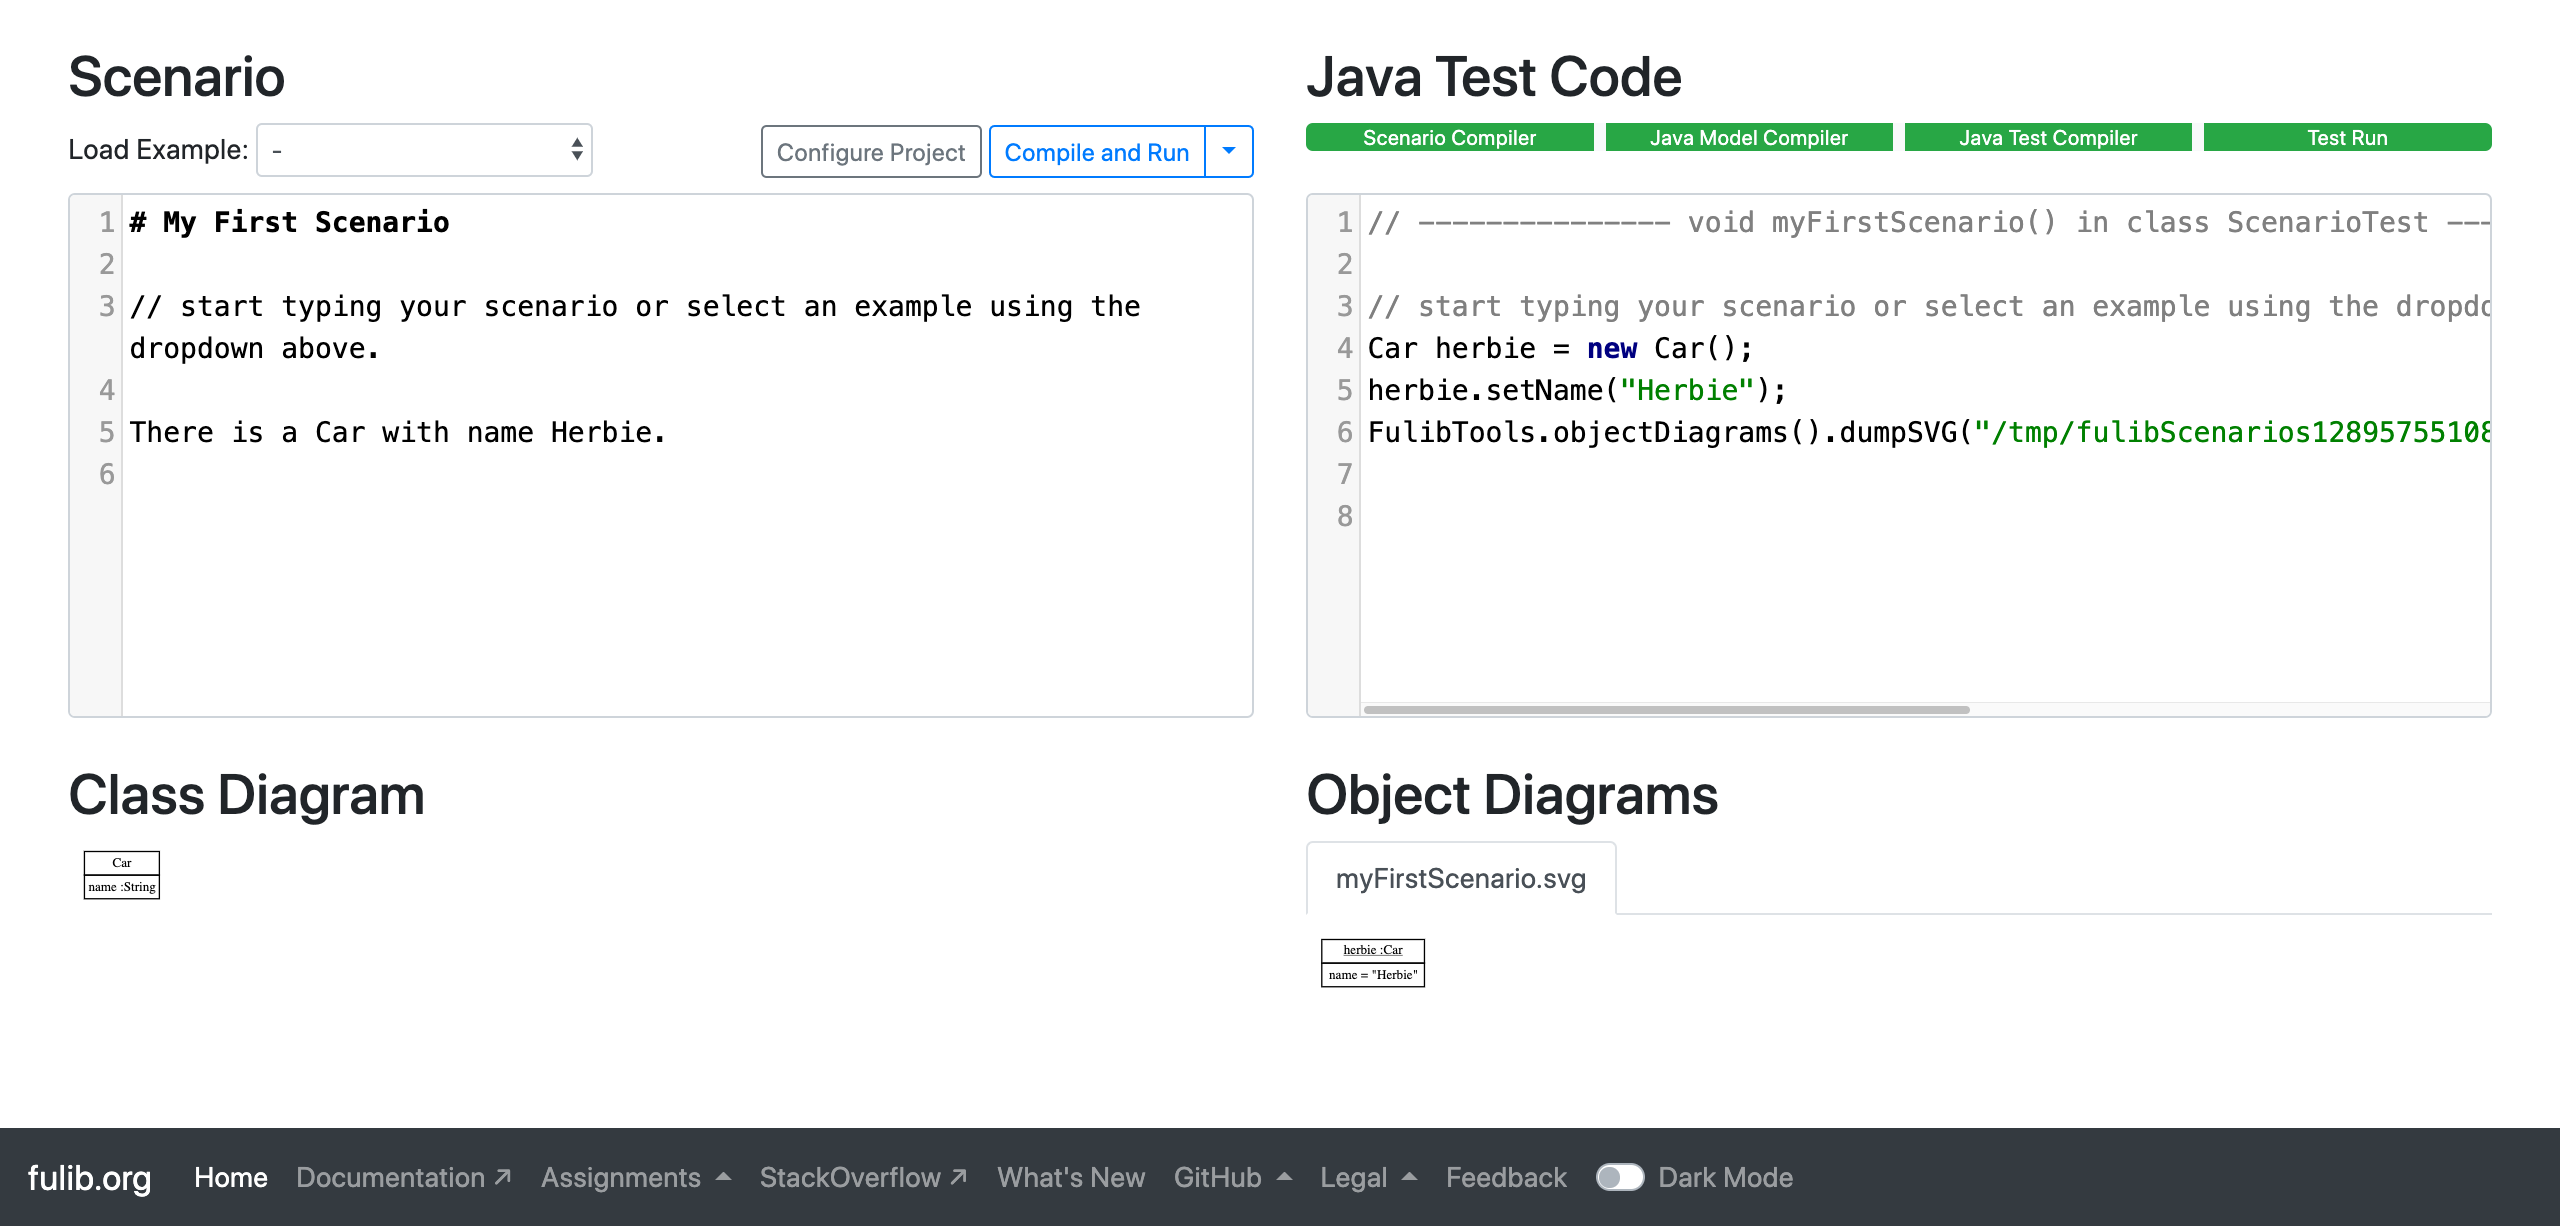
\includegraphics[width=\textwidth]{chapter/fulib.org/img/four-pane-editor.png}
    \caption{Der Vier-Panel-Editor auf der Hauptseite von fulib.org}
    \label{fig:four-pane-editor}
\end{figure}

Dieser zeigt oben links den Scenario-Editor sowie darüber dessen Toolbar.
Oben rechts gibt es ein Fenster für den generierten Java-Code, das auch die Konsolenausgabe des Compilers enthält.
Darüber zeigt eine Statusleiste, welche ob das Kompilieren und Ausführen erfolgreich war und wenn nicht, welches Tool fehlgeschlagen ist.
Im unteren Teil werden links das Klassendiagramm und rechts Objektdiagramme dargestellt.

Am unteren Rand der Seite befindet sich stets der Footer.
Dieser enthält Links zur Navigation innerhalb der Seite und zu externen Referenzen.
Außerdem finden sich darunter die Einstellungen für Datenschutz,
Möglichkeiten zum Hinterlassen von Feedback und zum Einsehen von Änderungen,
und die Schaltfläche zum Wechseln in den Nachtmodus.

\subsection{Interaktiver Spielplatz}\label{subsec:interactive-playground}

\todo{
Sofortiges Feedback.
Komplettübersicht -> Klassen, Objekte, Code
}

\subsection{Tutorials}\label{subsec:tutorials}

\todo{
Aufsteigende Schwierigkeit.
Editierbarkeit -> Spielplatz.
}

\subsection{Projektstarter}\label{subsec:project-starter}

\todo{
Gradle.
}

\subsection{Sicht der Studenten}\label{subsec:students-view}

\todo{
Feedback-Funktion.
Allgemeine Bewertung (PM).
Wünsche.
}

\subsection{Datensammlung}\label{subsec:data-collection}

\todo{
Request-Logging.
Fehleranalyse.
Lernverlauf.
Privacy-Einstellungen.
}
